\documentclass[a4paper]{article}
\usepackage[a4paper,top=2cm,bottom=2.5cm,left=1.5cm,right=1.5cm,marginparwidth=1.75cm]{geometry}
%% Language and font encodings
\usepackage[english]{babel}
\usepackage[utf8x]{inputenc}
\usepackage{listings}

%% Sets page size and margins

\usepackage{float}
%% Useful packages
\usepackage{amsmath}
\usepackage[colorinlistoftodos]{todonotes}
\usepackage[colorlinks=true, allcolors=blue]{hyperref}
\usepackage{listings}
\usepackage{url}
\usepackage{graphicx}
\graphicspath{ {./images/} }
% \DeclareGraphicsExtensions{.pdf,.jpg,.png}

%% defined colors
\definecolor{Blue}{rgb}{0,0,0.5}
\definecolor{Green}{rgb}{0,0.75,0.0}
\definecolor{LightGray}{rgb}{0.6,0.6,0.6}
\definecolor{DarkGray}{rgb}{0.3,0.3,0.3}

\title{\textbf{Lempel-Ziv Compression With Random Access} }
\author{
Shaik Mastan Vali, Srikanth Kamparaju\\
Supervisor - Dr. Shashank Vatedka 
%  \\ \textbf{Group} 1234
}
\date{}


\begin{document}
\maketitle
\section{Introduction}
In the last decade, the amount of data generated has increased dramatically. Data from genetics, video data, virtual reality, and other fields is exploding at an unprecedented rate. This data avalanche has necessitated the development of more effective compression methods for data storage and management. Data storage, on the other hand, is no longer for archival purposes. In modern applications, the majority of the stored data must be retrieved and analysed on a regular basis in order to make statistical choices. This has prompted the development of a new class of data compressors: efficient compressors that allow for computation on the compressed data while remaining rate efficient. shows up when source sequences are very long. In other words, to query a single source symbol,traditional algorithms require accessing a number of stored bits that scale with the length of the sequence. So asymptotically, as the sequence length n tends to infinity, one needs to access a large number of stored bits (scaling with n) to query a single bit.We are interested in constructions that allow close-to-optimal compression with efficient random access. When the compression sizes are quite large, the ability to deal with the compressed data without first decompressing the dataset is especially important (say 100x). We've previously seen how they can help with a variety of issues. In the realm of genomics, for example, much effort has gone into developing compressors that efficiently compress the 2D-tabular variant-call dataset while also allowing for random decompression of any row or column.

We're looking for a way to save a source sequence with the fewest possible bits while yet permitting a query of any place in the sequence using only a few bits of the compressed sequence. To recover a single symbol using classic compressors like Lempel-Ziv based techniques, one must access the complete compressed sequence. This is desired since these algorithms' space efficiency becomes apparent when source sequences are quite long. To put it another way, standard algorithms involve accessing a number of stored bits that grow with the length of the sequence to query a single source symbol.As the sequence length n approaches infinity, accessing a large number of stored bits (scaling with n) is required to query a single bit.We're looking for data structures that allow for near-optimal compression while maintaining efficient random access.
\section{Problem Setup}

A sequence $X^{n}$ is generated from a stationary and ergodic source with alphabet $x$. We would like to losslessly store $X^{n}$ using the minimum expected number of bits such that every symbol $X_{i}, \mathrm{i}=0, \ldots, \mathrm{n-1}$, can be reliably reconstructed by accessing no more than to of the stored bits in the memory. A compression scheme with blocklength $\mathrm{n}$, random access $t^{(n)}$, and the rate $R^{(n)}$ is defined by an encoder:

$$
f^{(n)}: \boldsymbol{X}^{(n)} \rightarrow\{0,1\}^{*}
$$

And decoder pairs $\left(S_{i}^{(n)}, g_{i}^{(n)}\right)$ :

$$
\begin{gathered}
S_{i} \subseteq N,\left|S_{i}^{(n)}\right|=t^{(n)}, \\
g_{i}^{(n)}:\{0,1\}^{t^{(n)}} \rightarrow x, \forall i=0, \ldots, n-1
\end{gathered}
$$

such that the following are true:

$$
\begin{gathered}
R^{(n)}=\frac{E\left[f^{(n)}\left(X^{n}\right)\right]}{n}, \\
g^{(n)}\left(\left\{f^{(n)}\left(X^{(n)}\right)\right\}_{S_{i}^{(n)}}\right)=X_{i}
\end{gathered}
$$

Here, $\left\{f^{(n)}\left(X^{n}\right)\right\}_{S_{i}^{(n)}}$ denotes the subsequence of $f^{(n)}\left(X^{n}\right)$ that belongs to the positions in $S_{i}^{(n)}$. The pair $(R, t)$ is said to be achievable if there exists a sequence of compression schemes (indexed by $n$ ) such that

$$
\begin{array}{lll}
\lim _{n \rightarrow \infty} & R^{(n)} & \rightarrow R \\
\lim _{n \rightarrow \infty} & t^{(n)} & \rightarrow t
\end{array}
$$

In this work, We implement and compare the average random time vs compression size of three different compression schemes such as RLZ , Dense sparse and BV-RLZ 
\section{Compression Schemes }
\subsection{RLZ Compression}
In this scheme, we divide the file into fixed-size chunks and compress each chunk using lempel-ziv algorithm  both with  dictionary and without dictionary compression. 

\textbf{Compression:} The sequence $X$ is divided into blocks of length $b$ and is compressed block by block. Let the compressed length of the $i^{th}$ block be $L_i$ and the number of blocks be $N_b$. The header $h$ is stored as follows-
$$
\begin{gathered}
    h_i = \sum_{j=0}^{i} L_j, \text{ for } 0 \leq i \leq N_b - 1 \\
\end{gathered}
$$

\textbf{Decompression:} To access the $i^{th}$ block, the start position and the compressed size of the block is obtained from the header as follows-
$$
\begin{gathered}
    start_i = h_i \\
    size_i = h_{i+1} - h_i,  \text{ for } 0 \leq i \leq N_b - 1 \\
\end{gathered}
$$
Using these values, the block can be accessed and decompressed.


\subsection{Dense-Sparse stream based compression}
In this scheme, the file $X$ is divided into fixed-size chunks and each chunk is stored using two streams: dense stream $D$ and sparse stream $S$. This scheme is a modified version of [1]. \\
\textbf{Compression:} Let $C_i$ be the compressed block corresponding to the original block $B_i$, and $L_i$ be the length of $C_i$. The typicality of the block is decided using the threshold $T = b (H(X) + \epsilon)$.
\begin{itemize}
    \item If $C_i \leq T $, then \\~\\
         \smallskip \hspace{5ex}$
        \begin{gathered}
            D_i = C_i[0 \ldots L_i-1] \\
            S_i = 0 ^ b
        \end{gathered}
        $
    \item Else,\\~\\
        \smallskip \hspace{5ex} $
        \begin{gathered}
            D_i = C_i[0 \ldots T-1] \\
            S_i = C_i[T \ldots L_i-1]
        \end{gathered}
        $
\end{itemize}
Each of $D_i$ and $S_i$ are padded with zeroes such that the length of $D_i$ is $T$ and the length of $S_i$ is $b$. 
Finally, the sparse stream $S$ is compressed using a sparse bit-vector compressor.

The header $h$ is stored as follows-
$$
\begin{gathered}
    h_i = \sum_{j=0}^{i} L_j, \text{ for } 0 \leq i \leq N_b - 1 \\
\end{gathered}
$$

\textbf{Decompression:} To decompress the $i^{th}$ block, the LZ-compressed block $C_{i}^{'}$ needs to be constructed. The start position and the compressed size of the block is obtained from the header as follows-
$$
\begin{gathered}
    start_i = h_i \\
    size_i = h_{i+1} - h_i,  \text{ for } 0 \leq i \leq N_b - 1 \\
\end{gathered}
$$
The compressed block $C_{i}^{'}$ is constructed as follows-
\begin{itemize}
    \item If $size_i \leq T $, then \\~\\
         \smallskip \hspace{5ex}$
        \begin{gathered}
            C_i ^ {'} = D[0 \ldots size_i - 1]
        \end{gathered}
        $ 
    \item Else,\\~\\
         \smallskip \hspace{5ex}$
        \begin{gathered}
            C_i ^ {'} = D[0 \ldots T - 1] \quad || \quad S[0 \ldots size_i - T - 1]
        \end{gathered}
        $
        
        where $||$ is the concatenation operator.
\end{itemize}
The sparse stream values are accessed using the random access operator on the sparse bit-vector.
The block $C_i ^ {'}$ can now be decompressed using the Lempel-Ziv algorithm to obtain $B_i$.
\subsection{BV-RLZ compression}
In this scheme, the file is divided into fixed-size chunks and each chunk is compressed, same as in the RLZ scheme. The header is stored as a compressed bit-vector.

\textbf{Compression:} The sequence $X$ is divided into blocks of length $b$ and is compressed block by block. Let the compressed length of the $i^{th}$ block be $L_i$. The header $h$ is stored using the bit-vector data structure. Let $pos$ be defined as -
$$
\begin{gathered}
    pos_i = \sum_{j=0}^{i} L_j, \text{ for } 0 \leq i \leq N_b - 1 \\
\end{gathered}
$$
Let $L_X = \sum_{j=0}^{N_b - 1} L_i$ be the size of the compressed file.
Initially, $h = 0^{L_X}$. The bits of $h$ are set as follows-
$$
\begin{gathered}
    h_{pos_i} = 1, \text{ for } 0 \leq i \leq N_b - 1
\end{gathered}
$$
The bit-vector $h$ is compressed using the sparse bit-vector compressor.

\textbf{Decompression:} To access the $i^{th}$ block, the start position and the compressed size of the block is obtained from the header as follows-
$$
\begin{gathered}
    start_i = select_h(i + 1) \\
    size_i = select_h(i + 2) - select_h(i + 1),  \text{ for } 0 \leq i \leq N_b - 1 \\
\end{gathered}
$$
where $select_h(i)$ is the standard select operator on the compressed bit-vector $h$.
Using these values, the compressed block can be constructed and decompressed using the LZ algorithm.


\section{Experiments and Results}
The three compression schemes were tested on the Wikipedia corpus (enwik8, enwik9), IMDB principal data and a protein FASTA file both with and without using a dictionary. The ZSTD library was used for LZ compression and SDSL library was used for bit-vector compression. The experiments were run on Linux machine having Ubuntu 20.04.3 LTS and AMD EPYC 7452 32-Core Processor with 128GiB RAM. All the methods were implemented in C++14 and compiled using g++ 9.3.0. 

The values of chunk size $b$ used were in the range $[fileSize / 10000, fileSize / 1000]$, where $fileSize$ is the size of the original file. The value of $\epsilon$ for the threshold used was $0.01$.

\begin{figure}[H]
    \centering
    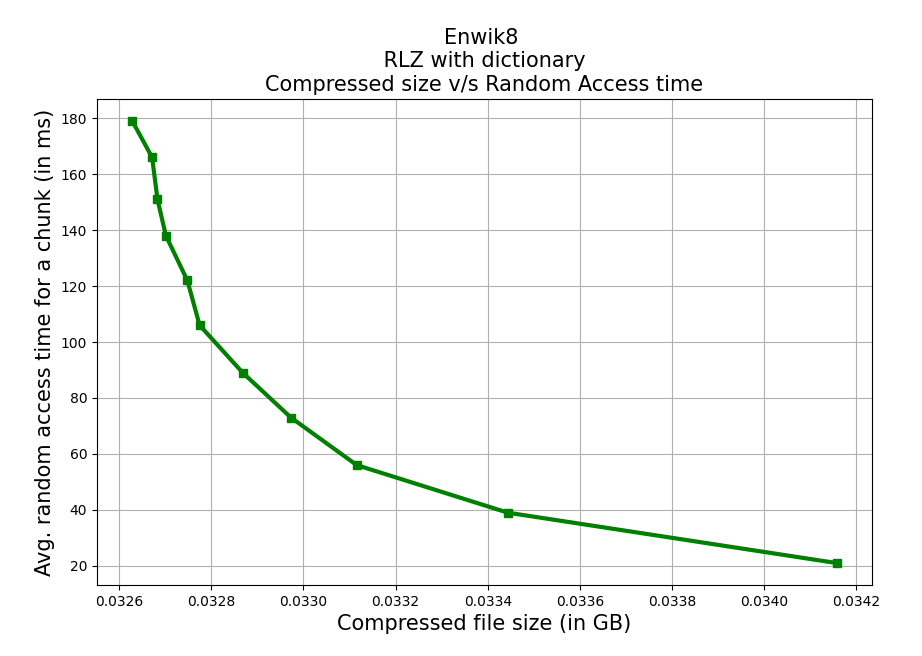
\includegraphics[width=\textwidth/2]{Figs/Enwik8_RLZ_dict.png}
    \caption{Compressed size v/s random access time for RLZ scheme with dictionary}
    \label{fig:enwik8_rlz_dict}
\end{figure}

\begin{figure}[H]
    \centering
    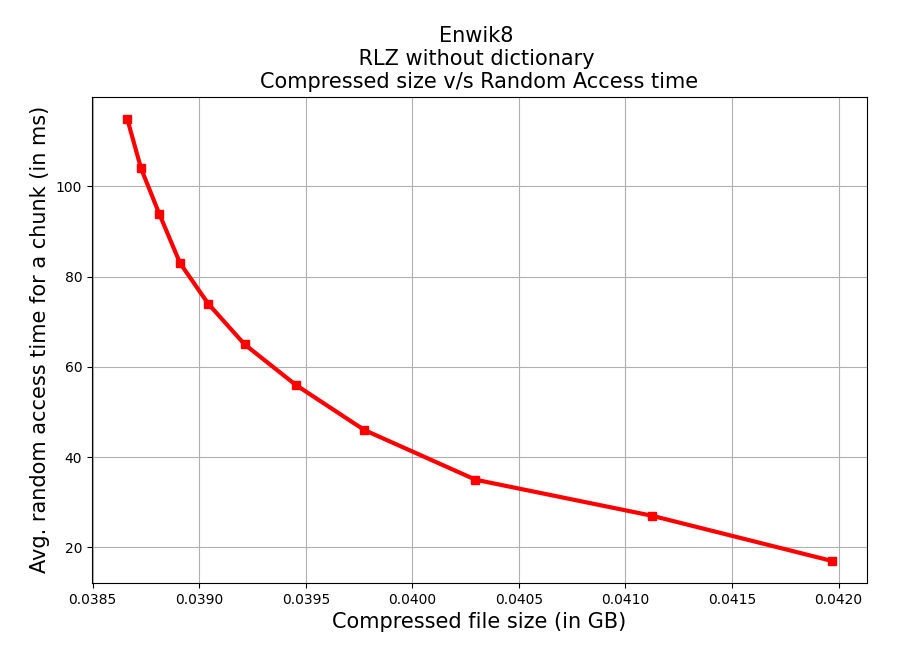
\includegraphics[width=\textwidth/2]{Figs/Enwik8_RLZ_nodict.png}
    \caption{Compressed size v/s random access time for RLZ scheme without dictionary}
    \label{fig:enwik8_rlz_nodict}
\end{figure}

From \href{fig:enwik8_rlz_dict}{fig-1} and \href{fig:enwik8_rlz_nodict}{fig-2} it can be observed that the RLZ scheme using a dictionary gives a smaller compressed file, but consumes more time for random access due to the additional overhead.

\begin{figure}[H]
    \centering
    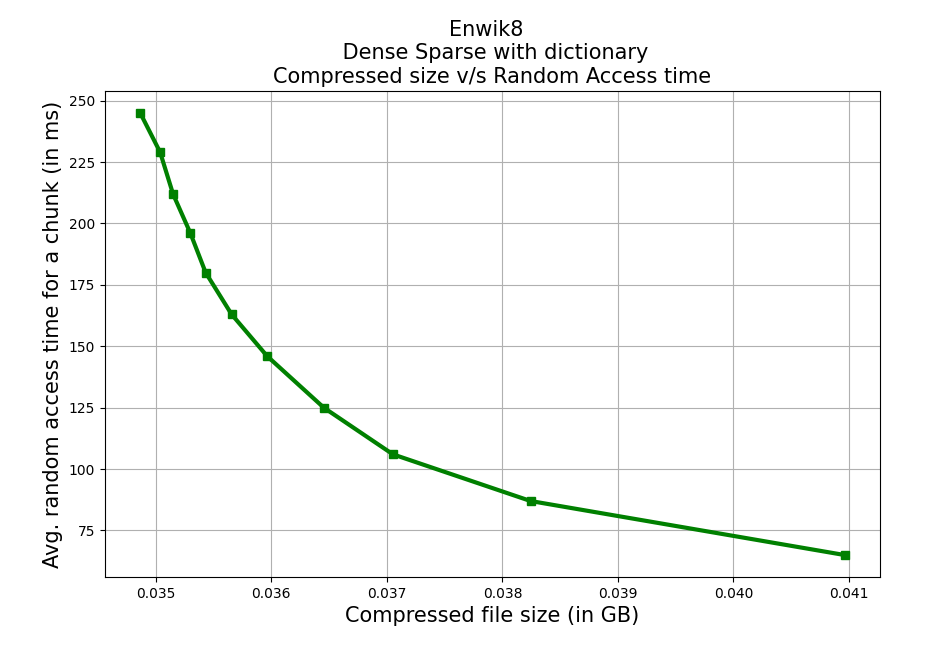
\includegraphics[width=\textwidth/2]{Figs/Enwik8_DS_dict.png}
    \caption{Compressed size v/s random access time for Dense-sparse scheme with dictionary}
    \label{fig:enwik8_ds_dict}
\end{figure}
\begin{figure}[H]
    \centering
    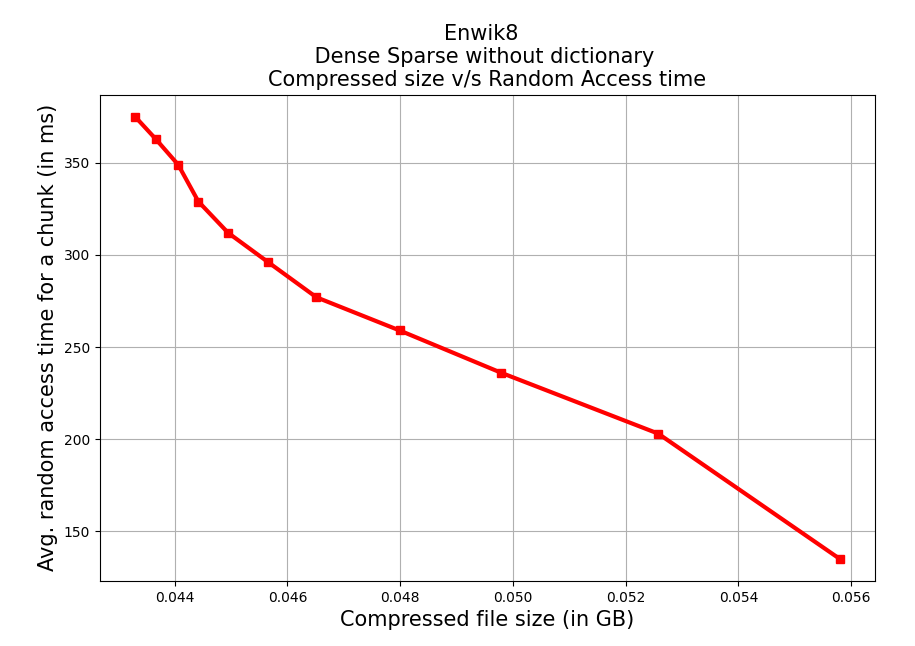
\includegraphics[width=\textwidth/2]{Figs/Enwik8_DS_nodict.png}
    \caption{Compressed size v/s random access time for Dense-sparse scheme without dictionary}
    \label{fig:enwik8_ds_nodict}
\end{figure}
From \href{fig:enwik8_ds_dict}{fig-3} and \href{fig:enwik8_ds_nodict}{fig-4} it can be observed that the dense-sparse scheme using a dictionary gives a smaller compressed file and consumes less time for random access, because of the smaller compressed size of each chunk and thereby less random access time.

\begin{figure}[H]
    \centering
    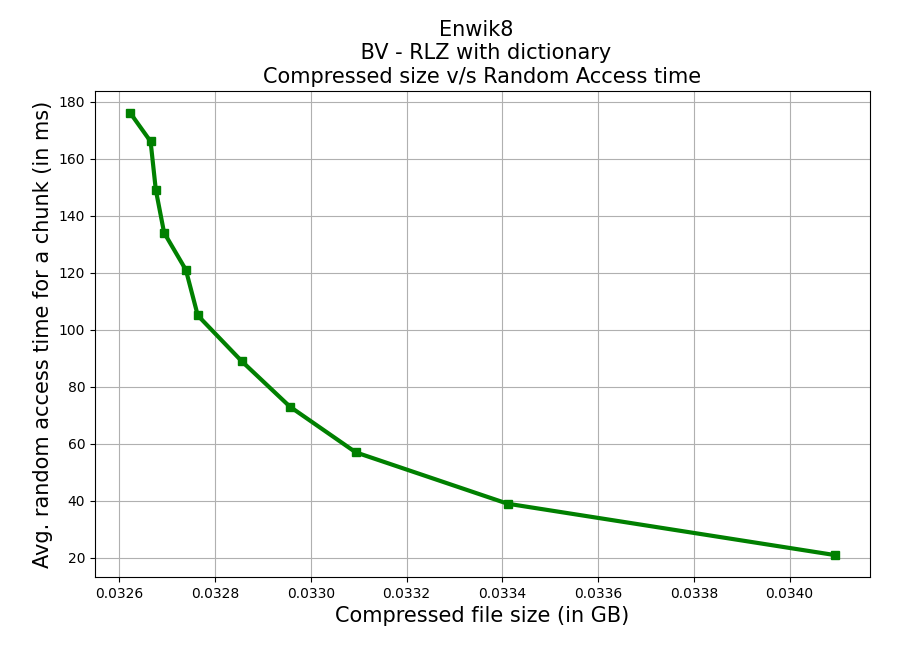
\includegraphics[width=\textwidth/2]{Figs/Enwik8_BV_RLZ_dict.png}
    \caption{Compressed size v/s random access time for BV-RLZ scheme with dictionary}
    \label{fig:enwik8_bv_rlz_dict}
\end{figure}


\begin{figure}[H]
    \centering
    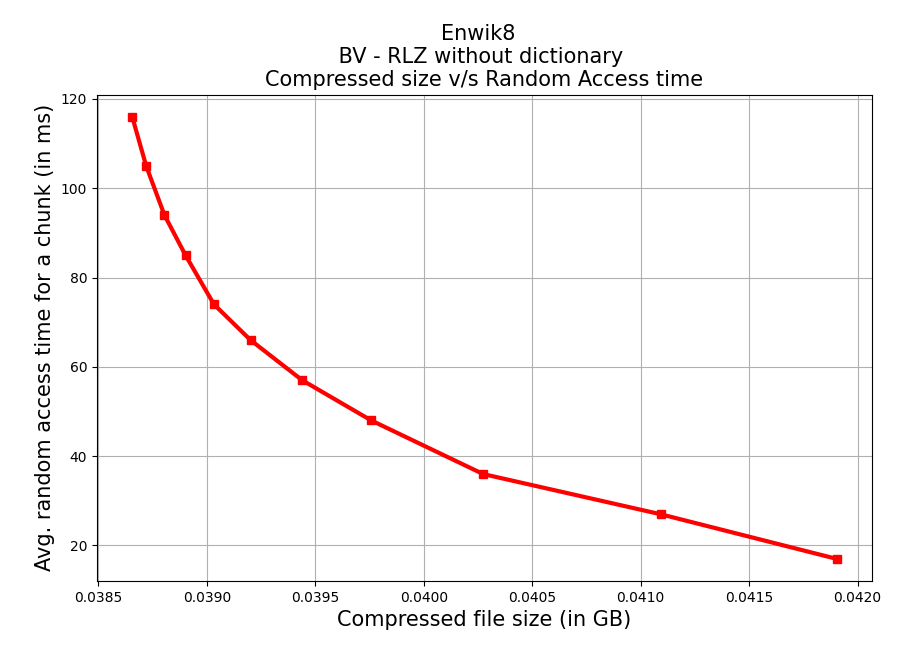
\includegraphics[width=\textwidth/2]{Figs/Enwik8_BV_RLZ_nodict.png}
    \caption{Compressed size v/s random access time for BV-RLZ scheme without dictionary}
    \label{fig:enwik8_bv_rlz_nodict}
\end{figure}

From \href{fig:enwik8_bv_rlz_dict}{fig-5} and \href{fig:enwik8_bv_rlz_nodict}{fig-6} a conclusion similar to the RLZ scheme can be derived.
\\~\\
Further, a custom method \verb|get(start, length)| was implement to optimize the random access time in dense-sparse scheme. The method returns the subsequence $Y[start \ldots start + length - 1]$ from $C_Y$, where $C_Y$ is the compressed bit-vector corresponding to the bit-vector $Y$. Suppose that we need to access a subsequence of length $k$ in the compressed bit-vector $C_Y$. Traditionally, using the random access operator \verb|[]| pre-defined in the SDSL library, the number of computations required is $\mathcal{O}(k (t_{select} + n / m))$ , where $m$ is the number of zeroes in the original bit vector $Y$. The custom method achieves this using $\mathcal{O}(t_{select} + kn / m)$ computations by using a single \verb|select()| method call.

\begin{figure}[H]
    \centering
    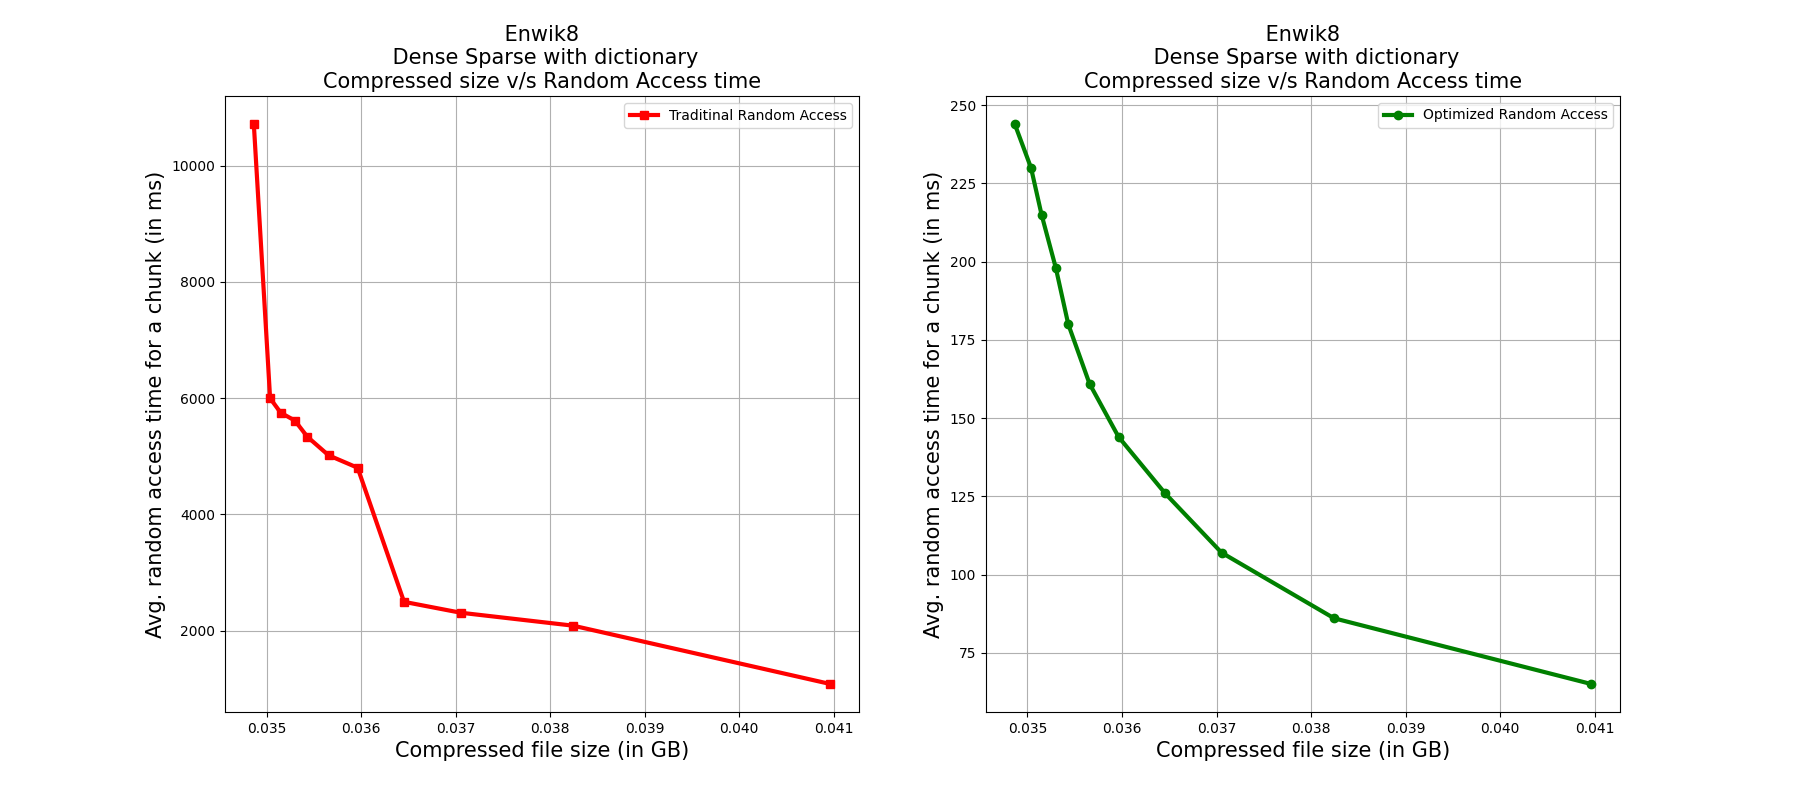
\includegraphics[width=\textwidth]{Figs/ds_opt.png}
    \caption{Compressed size v/s random access time for dense-sparse scheme using the traditional and optimized random access}
    \label{fig:ds_opt}
\end{figure}

From \href{fig:ds_opt}{fig-7}, a significant improvement in random access time can be observed using the optimized random access, while the compressed file size remains same. 

The source codes, instructions to run and text file links are in the following \href{https://github.com/srikanth2001/IDP_EE4015}{repository}
\section{References}
\begin{enumerate}
  \item K.Tatwawadi, Shirin Saeedi Bidokhti, Tsachy Weissman, "On Universal Compression with Constant Random Access"
  \item Thomas M Cover, Joy A Thomas, "Elements of Information Theory" \texttt{enumerate} environment.
  \item Kewen Liao, et al, "Effective Construction of Relative Lempel-Ziv Dictionaries"
  \item \href{http://facebook.github.io/zstd/}{Zstandard - Real-time data compression algorithm} 
  \item \href{https://zstd.docsforge.com/dev/}{Getting Started - Zstd dev} 
  \item \href{https://github.com/simongog/sdsl-lite}{SDSL library}
\end{enumerate}
\end{document}